% Template for PLoS
% Version 3.5 March 2018
%
% % % % % % % % % % % % % % % % % % % % % %
%
% -- IMPORTANT NOTE
%
% This template contains comments intended 
% to minimize problems and delays during our production 
% process. Please follow the template instructions
% whenever possible.
%
% % % % % % % % % % % % % % % % % % % % % % % 
%
% Once your paper is accepted for publication, 
% PLEASE REMOVE ALL TRACKED CHANGES in this file 
% and leave only the final text of your manuscript. 
% PLOS recommends the use of latexdiff to track changes during review, as this will help to maintain a clean tex file.
% Visit https://www.ctan.org/pkg/latexdiff?lang=en for info or contact us at latex@plos.org.
%
%
% There are no restrictions on package use within the LaTeX files except that 
% no packages listed in the template may be deleted.
%
% Please do not include colors or graphics in the text.
%
% The manuscript LaTeX source should be contained within a single file (do not use \input, \externaldocument, or similar commands).
%
% % % % % % % % % % % % % % % % % % % % % % %
%
% -- FIGURES AND TABLES
%
% Please include tables/figure captions directly after the paragraph where they are first cited in the text.
%
% DO NOT INCLUDE GRAPHICS IN YOUR MANUSCRIPT
% - Figures should be uploaded separately from your manuscript file. 
% - Figures generated using LaTeX should be extracted and removed from the PDF before submission. 
% - Figures containing multiple panels/subfigures must be combined into one image file before submission.
% For figure citations, please use "Fig" instead of "Figure".
% See http://journals.plos.org/plosone/s/figures for PLOS figure guidelines.
%
% Tables should be cell-based and may not contain:
% - spacing/line breaks within cells to alter layout or alignment
% - do not nest tabular environments (no tabular environments within tabular environments)
% - no graphics or colored text (cell background color/shading OK)
% See http://journals.plos.org/plosone/s/tables for table guidelines.
%
% For tables that exceed the width of the text column, use the adjustwidth environment as illustrated in the example table in text below.
%
% % % % % % % % % % % % % % % % % % % % % % % %
%
% -- EQUATIONS, MATH SYMBOLS, SUBSCRIPTS, AND SUPERSCRIPTS
%
% IMPORTANT
% Below are a few tips to help format your equations and other special characters according to our specifications. For more tips to help reduce the possibility of formatting errors during conversion, please see our LaTeX guidelines at http://journals.plos.org/plosone/s/latex
%
% For inline equations, please be sure to include all portions of an equation in the math environment.  For example, x$^2$ is incorrect; this should be formatted as $x^2$ (or $\mathrm{x}^2$ if the romanized font is desired).
%
% Do not include text that is not math in the math environment. For example, CO2 should be written as CO\textsubscript{2} instead of CO$_2$.
%
% Please add line breaks to long display equations when possible in order to fit size of the column. 
%
% For inline equations, please do not include punctuation (commas, etc) within the math environment unless this is part of the equation.
%
% When adding superscript or subscripts outside of brackets/braces, please group using {}.  For example, change "[U(D,E,\gamma)]^2" to "{[U(D,E,\gamma)]}^2". 
%
% Do not use \cal for caligraphic font.  Instead, use \mathcal{}
%
% % % % % % % % % % % % % % % % % % % % % % % % 
%
% Please contact latex@plos.org with any questions.
%
% % % % % % % % % % % % % % % % % % % % % % % %

\documentclass[10pt,letterpaper]{article}
\usepackage[top=0.85in,left=2.75in,footskip=0.75in]{geometry}

% amsmath and amssymb packages, useful for mathematical formulas and symbols
\usepackage{amsmath,amssymb}

% Use adjustwidth environment to exceed column width (see example table in text)
\usepackage{changepage}

% Use Unicode characters when possible
\usepackage[utf8x]{inputenc}

% textcomp package and marvosym package for additional characters
\usepackage{textcomp,marvosym}

% cite package, to clean up citations in the main text. Do not remove.
\usepackage{cite}

% line numbers
\usepackage[right]{lineno}

% Use nameref to cite supporting information files (see Supporting Information section for more info)
\usepackage{xr-hyper}%for cross ref in overleaf
\usepackage{nameref,hyperref}
%always load hyperref last

% ligatures disabled
\usepackage{microtype}
\DisableLigatures[f]{encoding = *, family = * }

% color can be used to apply background shading to table cells only
\usepackage[table,dvipsnames]{xcolor}

% array package and thick rules for tables
\usepackage{array}

%strikethrough
\usepackage{soul}

%sara: for commenting the pdf to add alt text (if anyone knows a better solution for atl text please help)
\usepackage{pdfcomment}

%Janani: for inserting sparingly few super relevant emojis
% \usepackage{emoji} %Rocio: https://www.overleaf.com/learn/latex/Questions/Inserting_emojis_in_LaTeX_documents_on_Overleaf#Emoji_characters_and_the_Overleaf_editor

% create "+" rule type for thick vertical lines
\newcolumntype{+}{!{\vrule width 2pt}}

% create \thickcline for thick horizontal lines of variable length
\newlength\savedwidth
\newcommand\thickcline[1]{%
  \noalign{\global\savedwidth\arrayrulewidth\global\arrayrulewidth 2pt}%
  \cline{#1}%
  \noalign{\vskip\arrayrulewidth}%
  \noalign{\global\arrayrulewidth\savedwidth}%
}

% \thickhline command for thick horizontal lines that span the table
\newcommand\thickhline{\noalign{\global\savedwidth\arrayrulewidth\global\arrayrulewidth 2pt}%
\hline
\noalign{\global\arrayrulewidth\savedwidth}}


% Remove comment for double spacing
%\usepackage{setspace} 
%\doublespacing

% Text layout
\raggedright
\setlength{\parindent}{0.5cm}
\textwidth 5.25in 
\textheight 8.75in

% Bold the 'Figure #' in the caption and separate it from the title/caption with a period
% Captions will be left justified
\usepackage[aboveskip=1pt,labelfont=bf,labelsep=period,justification=raggedright,singlelinecheck=off]{caption}
\renewcommand{\figurename}{Fig}

% Use the PLoS provided BiBTeX style
\bibliographystyle{plos2015}

% Remove brackets from numbering in List of References
\makeatletter
\renewcommand{\@biblabel}[1]{\quad#1.}
\makeatother



% Header and Footer with logo
\usepackage{lastpage,fancyhdr,graphicx}
\usepackage{epstopdf}
%\pagestyle{myheadings}
\pagestyle{fancy}
\fancyhf{}
%\setlength{\headheight}{27.023pt}
%\lhead{\includegraphics[width=2.0in]{PLOS-submission.eps}}
\rfoot{\thepage/\pageref{LastPage}}
\renewcommand{\headrulewidth}{0pt}
\renewcommand{\footrule}{\hrule height 2pt \vspace{2mm}}
\fancyheadoffset[L]{2.25in}
\fancyfootoffset[L]{2.25in}
\lfoot{\today}

%% Include all macros below

\newcommand{\lorem}{{\bf LOREM}}
\newcommand{\ipsum}{{\bf IPSUM}}

%% END MACROS SECTION


\begin{document}

\vspace*{0.2in}

% Title must be 250 characters or less.
\begin{flushleft}
{\Large
\textbf\newline{Ten simple rules to host an inclusive conference} % Please use "sentence case" for title and headings (capitalize only the first word in a title (or heading), the first word in a subtitle (or subheading), and any proper nouns).
}
\newline
% Insert author names, affiliations and corresponding author email (do not include titles, positions, or degrees).
\\
Rocío Joo\textsuperscript{1*\Yinyang}, 
Andrea Sánchez-Tapia\textsuperscript{2\Yinyang},
Sara Mortara\textsuperscript{3},
Yanina Bellini Saibene\textsuperscript{4,5},
Heather Turner\textsuperscript{6}, %\ddag},
Dorothea Hug Peter\textsuperscript{7}, %\ddag},
Natalia Soledad Morandeira\textsuperscript{8},
Matt Bannert\textsuperscript{9},
Batool Almazrouq\textsuperscript{10},
Elizabeth Hare\textsuperscript{11},
Laura Ación\textsuperscript{5,12},
Juan Pablo Narváez-Gómez\textsuperscript{13},
Marcela Alfaro Córdoba\textsuperscript{14},
Federico Marini\textsuperscript{15},
Rita Giordano\textsuperscript{16},
Silvia Canelón\textsuperscript{17},
Anicet Ebou\textsuperscript{18},
Adithi Upadhya\textsuperscript{19},
Joselyn Chávez\textsuperscript{20},
Janani Ravi\textsuperscript{21*}
%,3\textcurrency}
\\
\bigskip
\textbf{1} Global Fishing Watch, Washington, DC 20036, USA
\\
\textbf{2} Instituto de Pesquisas Jardim Botânico do Rio de Janeiro, Rio de Janeiro, Rio de Janeiro, Brazil
\\
\textbf{3} International Institute for Sustainability, Rio de Janeiro, Rio de Janeiro, Brazil
\\
\textbf{4} Instituto Nacional de Tecnología Agropecuaria, Ruta Nac. N° 5, Km. 580, Anguil, La Pampa, Argentina; Universidad Nacional Guillermo Brown, Buenos Aires, Argentina
\\
\textbf{5} MetaDocencia, Argentina
\\
\textbf{6} Department of Statistics, University of Warwick, Coventry, UK; The R Foundation
\\
\textbf{7} Swiss Federal Institute for Forest, Snow and Landscape Research WSL, Birmensdorf, Switzerland
\\
\textbf{8} Instituto de Investigación e Ingeniería Ambiental, Universidad Nacional de San Martín - Consejo Nacional de Investigaciones Científicas y Técnicas, General San Martín, Buenos Aires, Argentina
\\
\textbf{9} KOF Swiss Economic Institute, ETH Zurich, Zurich, Switzerland
\\
\textbf{10} Institute of Systems, Molecular and Integrative Biology, University of Liverpool, Liverpool, L69 7ZB, UK; King Abdullah International Medical Research Center, Riyadh, Saudi Arabia
\\
\textbf{11} Dog Genetics LLC, Astoria, NY, USA
\\
\textbf{12} Instituto de Cálculo, FCEyN, UBA-CONICET, Buenos Aires, Argentina
\\
\textbf{13} Departamento de Botânica, Instituto de Biociências, Universidade de São Paulo, São Paulo, São Paulo, Brasil
\\
\textbf{14} Department of Statistics, University of California, Santa Cruz, CA, USA
\\
\textbf{15} Institute of Medical Biostatistics, Epidemiology and Informatics (IMBEI), University Medical Center Mainz, Mainz, Germany
\\
\textbf{16} Royal Society of Chemistry, Thomas Graham House (290), Science Park, Milton Road, Cambridge, UK
\\
\textbf{17} Department of Biostatistics, Epidemiology \& Informatics, University of Pennsylvania, Philadelphia, PA, USA.
\\
\textbf{18} Bioinformatics team, Département de Formation et de Recherches en Agriculture et Ressources Animales, Institut National Polytechnique Félix Houphouët-Boigny, BP 1313 Yamoussoukro, Côte d’Ivoire.
\\
\textbf{19} ILK Labs, Bengaluru, Karnataka, 560046, India
\\
\textbf{20} Instituto de Biotecnología, UNAM, Cuernavaca, Morelos, México
\\
\textbf{21} Departments of Pathobiology and Diagnostic Investigation, Microbiology and Molecular Genetics, Michigan State University, East Lansing, MI 48824, USA
\\
\bigskip

% Insert additional author notes using the symbols described below. Insert symbol callouts after author names as necessary.
% 
% Remove or comment out the author notes below if they aren't used.
%
% Primary Equal Contribution Note
\Yinyang Co-primary authors with equal contribution.

% Additional Equal Contribution Note
% Also use this double-dagger symbol for special authorship notes, such as senior authorship.
% \ddag These authors also contributed equally to this work.

% Current address notes
% \textcurrency Current Address: Dept/Program/Center, Institution Name, City, State, Country % change symbol to "\textcurrency a" if more than one current address note
% \textcurrency b Insert second current address 
% \textcurrency c Insert third current address

% Deceased author note
% \dag Deceased

% Use the asterisk to denote corresponding authorship and provide email address in note below.
*Co-corresponding authors: rocio.joo@globalfishingwatch.org, janani@msu.edu

\end{flushleft}
% Please keep the abstract below 300 words
\section*{Abstract}

Conferences are spaces to meet and to network within and across academic and technical fields, to learn about new advances, and share our work. They can help define career paths and create long-lasting collaborations and opportunities. 
However, these opportunities are not equal for all. 
This article introduces ten simple rules to host an inclusive conference based on the authors' recent experience organizing the 2021 edition of the useR! statistical computing conference, which attracted a broad range of participants from academia, industry, government, and the non-profit sector. 
Coming from different backgrounds, career stages, and even continents, we embraced the challenge of organizing a high-quality virtual conference in the context of the COVID-19 pandemic and making it a kind, inclusive, and accessible experience for as many people as possible.
The rules result from our lessons learned before, during, and after the organization of the conference. 
They have been written mainly for potential organizers and selection committees of conferences and contain multiple practical tips to help a variety of events become more accessible and inclusive. We see this as a starting point for conversations and efforts towards building more inclusive conferences across the world.
\hl{* Translated versions of the English abstract and the list of rules are available in ten languages in the Supporting Information: Arabic, French, German, Italian, Japanese, Korean, Portuguese, Spanish, Tamil, and Thai.}

% % Please keep the Author Summary between 150 and 200 words

\linenumbers

\section*{Introduction}

% Conferences are great, but only for some
Conferences are spaces to meet and reconnect with members from a specific community, learn about advances in the field, and share recent contributions.
A good conference experience can make a difference in the professional development of the participants and create long-lasting collaborations and opportunities. 
However, opportunities for participating in conferences are not equally available for all. 
Many academic and tech conferences have been spaces that reproduce systemic inequalities, by failing to overcome the barriers for participation and giving more opportunities to the most privileged individuals (typically white people from high-income backgrounds, prestigious institutions, \linelabel{power} native English speakers with no disabilities) \cite{arendDisparityConferenceRegistration2019, biggsAcademicConferenceChilly2018, depickerRethinkingInclusionDisability2020a, irishIncreasingParticipationUsing2020}.
\linelabel{background-a}Like many others, the authors of this article have experienced these inequalities in conferences, from different perspectives and levels of inclusion/exclusion and privilege. \linelabel{background-b}
We had the opportunity to organize a virtual and global statistical computing conference, useR! 2021 \cite{sanchez-tapia_user_2021-2}, for users and developers of the R programming language \cite{r_core_team_2021}.
Coming from different backgrounds, career stages, and even continents, we embraced the challenge of organizing a high-quality virtual conference in the context of the COVID-19 pandemic and making it a kind, inclusive, and accessible experience for as many people as possible.

% Roadmap of the paper
Here, we present a set of ten rules based on the lessons we learned before, during, and after the organization of the useR! conference.
\linelabel{methods-a} \hl{The rules were first drafted by the core team and the members of the diversity, accessibility, and inclusion team of useR! 2021 who wrote their own ten simple rules (see Supporting Information) based on the collective experience of organizing the conference and fueled by personal experiences and literature review.
A final list was proposed and then discussed and reviewed by the rest of the coauthors.} \linelabel{methods-b}
The rules are organized in three sections: three foundation rules, six design rules, and a continuity rule (\textbf{Fig. \ref{fig:diagram}}).
The \textbf{foundation rules} comprise key elements to conceive the work on diversity and inclusion in any conference. 
\textbf{Rule 1} is about setting a vision of diversity and inclusion that should guide all the efforts and decision making in the organization.
\textbf{Rule 2} focuses on how to create a safe and welcoming environment for all the attendees. 
\textbf{Rule 3} highlights the importance of starting with an inclusive and diverse organizing team and provides tips on work dynamics.
The \textbf{design rules} focus on weaving inclusion into the conference design process.
In \textbf{Rule 4}, we introduce multiple ways to counteract bias in the conference program (keynotes, program committee, abstract selection, and thematic sessions). 
\textbf{Rule 5} provides advice for designing an inclusive online component in virtual and hybrid conferences.
\textbf{Rule 6} focuses on accessibility practices to include people with disabilities.
In \textbf{Rule 7}, we provide suggestions to account for linguistic diversity. 
\textbf{Rule 8} offers tips for developing an inclusive communication strategy. 
In \textbf{Rule 9}, we address budgeting for inclusive practices and helping participants with affordable registration costs, scholarships, and other forms of financial support.
Finally, 
\textbf{Rule 10}, the \textbf{continuity} rule, emphasizes the importance of self-assessment and advocates for making the conference part of a long-term commitment to inclusion and for passing the torch to future organizers. 

We believe that these rules can guide organizers who intend to put inclusion at the core of their conference right from the conception and planning phases.
The rules will also help people who are part of meeting committees that oversee the site/location selection process, or that coordinate with the local organizers of conferences. 
We see the rules as a starting point for conversations and efforts towards building more inclusive conferences across the world.


% refs for past works in case we add them in line 311.
% %timperleyHeMoanaPukepuke2020, gewinWhatScientistsShould2019, brownAbleismAcademiaWhere2018, marks2021meeting
% some proposals for more inclusive conferences have been put into practice \cite{gichoraTenSimpleRules2010a, levitisCenteringInclusivityDesign2021, atkinsonJournalMedicine20202021, foramittiVirtuesVirtualConferences2021, ninerBetterWhomLeveling2021, rabyMovingAcademicConferences2021, numfocus_discover_2021},


\begin{figure}[!h]
\centering
%ast: use Adobe Acrobat to add missing accessibility metadata to your PDF file. ask how to do this this when submitting - some edits to the PDF may be needed to add alt-text to the final version https://chi2021.acm.org/for-authors/presenting/papers/guide-to-an-accessible-submission#late
\pdftooltip{
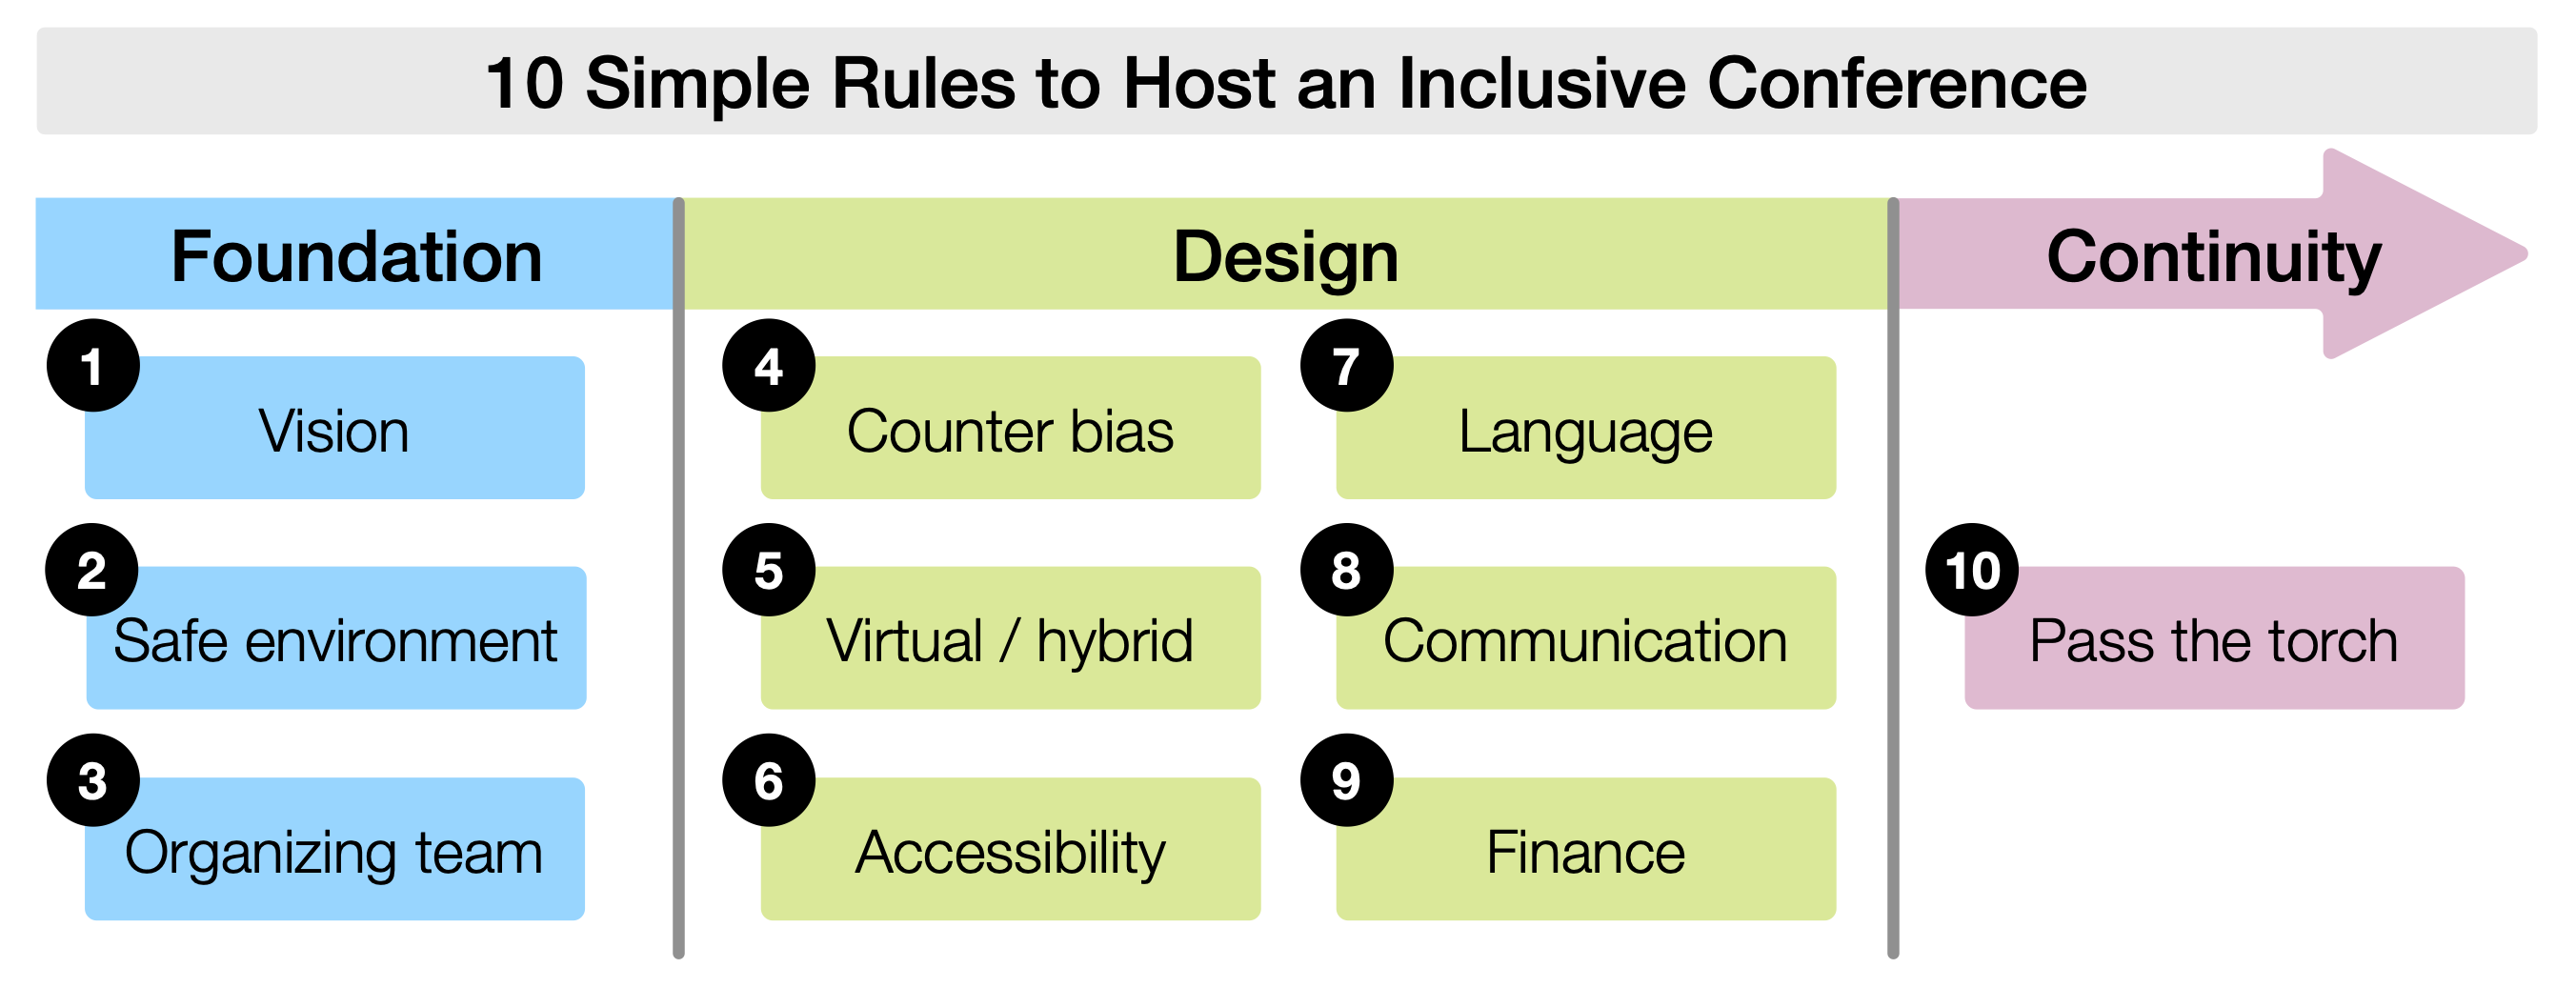
\includegraphics[width=\textwidth]{figs/fig1.png}}{
%Alt-text for the figure to be included in the final PDF: Diagram of how the 10 rules are organized into three groups: foundation rules (Rules 1-3), design rules (Rules 4 to 9), and a continuity rule (Rule 10). The overall diagram depicts an arrow from left to right which contains all the rules. In the left column, under the first label" Foundation", there are three text boxes in light blue: "1. Vision", "2. Safe environment", and "3. Organizing Team". In the middle column, under the label "Design Rules" there are six light green boxes with Rules "4. Counter bias", "5. Virtual / hybrid", "6. Accessibility", "7. Language", "8. Communication",  "9. Finance". To the right, below the arrowhead labeled Continuity, is the Tenth Rule in a light pink box "10. Pass the torch".
}
\caption{Schematic diagram of the rules organized in three groups: foundation (Rules 1, 2, and 3), design (Rules 4 to 9), and continuity (Rule 10).}
\label{fig:diagram}
\end{figure}


\section*{Rule 1: Set a vision for diversity and inclusion}
\label{rule_diversity}

Diversity encompasses multiple dimensions: age, disability, career stage, gender, gender identity, geographic origin, language, neurodiversity, race, religion, sexual orientation, and socioeconomic background, to name a few.
Human diversity should be celebrated and respected in every way. 
Nonetheless, we live in a world with implicit hierarchies along these axes. 
Some statuses (e.g. being cisgender, white, male, from North America or Western Europe) hold the privilege of being the defaults around which all systems—including conferences—are consciously and unconsciously built. 
People outside the dominant groups suffer different forms of oppression, like sexism, racism, ableism, homophobia, and transphobia, and sometimes these forms of oppression happen simultaneously and in complex ways (a concept known as `intersectionality' \cite{crenshawDemarginalizingIntersectionRace1989}).
As a result, some groups of people have been systematically excluded from or only partially included in academic, scientific, and professional circles.
Recognizing this systematic exclusion is paramount to inclusion.

\linelabel{indicators-1}\hl{
Lack of diversity will vary across areas of knowledge and depend on the geographic context of the conference.
Assess how it translates to the conference's particular field and scientific or professional community.
Some information can come from Diversity, Equity, and Inclusion (DEI) studies in the field or at a larger scale (e.g. STEM---science, technology, engineering, and mathematics) if they exist. 
Most importantly, involve the community---the subset of the general public that would ideally attend the conference---to help make this assessment and set the vision and goals of diversity and inclusion for the conference.} 
\linelabel{indicators-2}
Define measurable outcomes for these goals (e.g. a gender distribution of your speakers that is representative of the general population, the participation of people from diverse races and ethnicities among the organizers, speakers, and attendees, or participation from key geographic regions). 
They will help you be accountable along the way (see \textbf{Rule 10}). \linelabel{rule10} %\hl{and assess to what extent your inclusion goals were met (see \textbf{Rule 10})}.
The vision can be expressed in a diversity statement to be used as a reference for decision making in all areas of the conference organization.

\section*{Rule 2: Create a safe and welcoming environment}
\label{rule_inclusion}

% Inclusion for everyone
% Explain why we need this
Real inclusion can only be achieved in an environment where everybody feels safe, respected, and invited to take part in the conference activities and community. Be proactive and design a welcoming conference experience that takes into account the well-being of all the attendees. This means respecting all the aspects included in your diversity vision (see \textbf{Rule 1}). For example, promote the use and respect of pronouns and commit to respect all genders and sexual orientations. If the conference has an in-person component, pre-assign quiet, private spaces for religious practices, lactation, and child care. Include menu options that account for diverse dietary and religious requirements.
Some of these actions are very easy to implement and have a significant impact on making everyone feel truly included (see \cite{numfocus_discover_2021} for more examples and great advice on `low-hanging fruits'), some others need careful planning in advance, so it is good to have them in mind from the beginning.
Open the schedule for events organized by thematic groups and communities (e.g.\ task force meetings, LGBTQIA+-friendly spaces, Black in STEM\hl{, women in science}\linelabel{wis}), and sessions aimed to welcome first-timers to the conference.

% A culture of support (active bystandership) and code of conduct for a safe place 
Creating a safe and welcoming environment also requires promoting a culture of support, including the idea that anyone can intervene respectfully in defense of other attendees in case anything unpleasant, inappropriate, or offensive happens.
This is called `active bystandership'; consider providing training or pre-conference discussions to promote it.
However, the most important step that you should take to ensure the safety of the community is
adopting a code of conduct (CoC) and preparing a diverse response team to enforce it \cite{favaroYourScienceConference2016}.
\linelabel{unacceptable-1}The CoC is a living document meant to keep the community safe and should state clearly the behaviors that are deemed unacceptable by the community, the consequences for engaging in such behaviors, and the way to report violations \cite{auroraHowRespondCode2019}. 
\hl{Bear in mind that every dimension of diversity can be a target of unacceptable behavior. The CoC should help honor the vision expressed in the diversity statement.}\linelabel{unacceptable-2} 
 

The CoC response team must receive training on how to receive reports, respond to incidents, and communicate their responses to the whole community. The team should be prepared early during conference planning because CoC violations can happen before the conference begins (e.g.\ on social media or in organization meetings).  
Responding to CoC reports can be one of the most emotionally intense tasks of the team. Resources permitting, consider adding funds for their work to your budget (see \textbf{Rule 9}).
We strongly recommend reading `How to Respond to Code of Conduct Reports' \cite{auroraHowRespondCode2019} as an excellent starting point for building a strong CoC response team. 
 

\section*{Rule 3: Gather an inclusive and diverse organizing team}
\label{rule_organizing_team}

% Build a diverse team, and representation
A genuinely inclusive conference can only be organized by an inclusive and diverse team.
Organizers should comprise a team with people from as many different backgrounds as possible in terms of regions, genders, ethnicities, career stages, and other aspects of diversity.
People with disabilities often say: `Nothing about us without us' \cite{charlton_nothing_1998, werner_nothing_1998}; the same holds for other dimensions of diversity. 
Having people from diverse backgrounds in decision-making roles will positively affect the conference as a whole because all the processes will benefit from their expertise, experience, and distinct perspectives \cite{hongGroupsDiverseProblem2004}. 
The experience of people in marginalized groups
is especially important; they cannot be replaced by good intentions or second-hand knowledge from people who have not lived through the same experiences \cite{costanzachockDesign2020}.
In addition, a diverse team plays an essential role in creating a welcoming space because representation—seeing people with similar life experiences occupying critical positions of power and breaking negative stereotypes—is one of the best ways to create a sense of belonging for everyone participating in the conference.
\hl{If you have already started assembling an organizing team, check for gaps in its composition and do your best to fill them. 
The regional and local communities, groups, or associations in your field are good sources to tap into.}

\linelabel{subteam-1} \hl{Create sub-teams to distribute fairly the large amount of work that organizing a conference represents. 
Having a dedicated DEI team may be an excellent way to give the topic the attention and energy it requires.
The core team should support the DEI initiatives and advocate for inclusion across all conference areas.} \linelabel{subteam-2} 
It is important, though, to ensure that organizers with diverse backgrounds are not restricted to only work on diversity and inclusion aspects; 
every \hl{person} should have the freedom to choose which areas of the conference they want to contribute to.
When it comes to team leadership, do not expect self-nomination and voting to work as infallible mechanisms to fill these positions equitably. 
Instead, nominate folks directly and offer them leadership positions in the organizing team, especially those positions that would be typically occupied by people from privileged groups.
\hl{Moreover,} some people may lack the institutional or financial support to put time and effort into the organization tasks and do not have the luxury to commit for free; consider reallocating resources to give them a stipend for their work (see \textbf{Rule 9}).
In any case, try to find meaningful ways to acknowledge everybody's work. Use the conference spaces (e.g. webpage, opening/closing ceremony at the conference, social media) to give proper credit to the people who are making the event possible.
And most importantly, take care of your team and their well-being! Check on them regularly and make sure that everyone is comfortable. This represents a great amount of work and you will need to support each other for the long haul.


\section*{Rule 4: Consciously counteract bias in the conference program}
\label{rule_unbias}

\linelabel{invited}The conference program may lack diversity in the invited roles––-such as keynote speakers, program/scientific committee, session chairs, panelists––-, the accepted abstracts, and even the scope of the topics covered. 
It is important to counteract biases in all of these aspects.
When choosing or inviting people for visible and valued roles in the conference, it is likely that there will not be much diversity in the first pool of names \cite{dwyerNoticeWhoScience2021,swartzScienceValueDiversity2019,wongBuildDiversityScience2020,dignazioUnicornsJanitorsNinjas2020}.
Rather than deterring you, this should encourage you to go beyond your current networks to look for, reach out to, invite, encourage, and on-board great people that are not routinely in the spotlight, making sure that these roles do not reinforce existing privileges.\linelabel{invited-2}

Biases in the final list of abstracts begin with self-selection: some potential conference participants may not feel confident enough to submit their work, especially to large and prestigious conferences.
To mitigate such self-selection, some communities have pre-submission mechanisms to aid their members prepare and receive feedback for their abstract (e.g. the Latin-R and R-Ladies communities have volunteers to help their members improve their conference abstracts).
If this does not exist in your field yet, consider asking members of your community to provide a similar kind of mentorship.
\linelabel{multilingual-submission}\hl{To mitigate self-selection from non-native speakers, consider accepting submissions in several languages} (see \textbf{Rule 7}).\linelabel{multilingual-submission2}


The abstract review process can be subjected to implicit bias \cite{ross_everyday_2020} when folks in the selection committee unconsciously assign a positive or negative value to the names and affiliations of authors—and \linelabel{bias} their perceived origin, ethnicity, gender, or native language—, affecting the chances to get their work accepted.
Selection committees need to be reminded of such biases in the evaluation process, to try to avoid judging more scrupulously the work of people perceived as part of minoritized groups or being kinder when reviewing the abstracts from those perceived as part of privileged groups and considering their work as more relevant \cite{swartzScienceValueDiversity2019, andersson_implicit_2019}.
Evaluate the plausibility of anonymizing \hl{the submission information as much as possible}\linelabel{anonymous} and
define the most appropriate strategy for reviewing (e.g. double blind, double open, or single blind reviews; see \cite{numfocus_discover_2021}).
\linelabel{criteria-1} \hl{Even well-meaning and carefully crafted processes can be prone to reproduce the biases present in academia and society. It is, therefore, essential to examine the final list of selected abstracts to check if there is a lack of diversity. If proposals with similar quality were still judged differently because of unconscious bias, consider giving preference to the work from people in minoritized groups.
This manual examination at the final stage is unlikely to be reproducible. Nonetheless, the whole process should be as transparent as possible: evaluation criteria should be clearly stated and shared with the reviewers and authors, preferably during the call for abstracts.} \linelabel{criteria-2}
\linelabel{video-1}\hl{It is worth noting that self-selection and unconscious bias may be aggravated by the use of video abstracts as an alternative to written ones, affecting people without the resources to create good quality videos, people with disabilities, non-native speakers, racialized people, and people with diverse body types, among others.} \cite{spitschanVideoGrantProposals2021}\linelabel{video-2}

Bias can also be expressed in the level of visibility given to the diverse topics in the conference program.
In many academic or technological fields, typically competitive activities or areas---such as scientific publications or software development---are more valued than those focused on sharing and cooperation, like community building, teaching, or mentoring. 
The latter activities are equally, if not more, relevant and challenging, and are usually performed by women, racialized people, people with disabilities, and other minoritized groups \cite{cheng2020x+, burfordHomelinessMeantHaving2020, light_gender_2022}.
When planning the program for the conference, consider giving visibility to the whole range of activities and practitioners that contribute to the field by proposing new thematic sessions, broadening the scope of talks, keynotes, and tutorials. 


\section*{Rule 5: Design a strong online component} 
\label{rule_online}

After experiencing virtual conferences mostly due to the COVID-19 pandemic, there have been multiple calls to retain an online component in conferences, either as completely virtual events or using hybrid formats (combining in-person and online components) \cite{jooKeepOnlineOption2021, woolstonLearningLoveVirtual2020, ninerBetterWhomLeveling2021, roosOnlineConferencesNew2020, levitisCenteringInclusivityDesign2021, sarabipourChangingScientificMeetings2021}.
Virtual conferences remove barriers for inclusion like costs of participation, the logistics of long-distance and international travel, and discriminatory visa applications \cite{jooKeepOnlineOption2021, ninerBetterWhomLeveling2021, salibaGettingGripsOnline2020, gichoraTenSimpleRules2010a}. 
Make sure that you are not creating additional barriers when choosing conference platforms, schedule, and activities. 
Check every platform's screen reader accessibility (see \textbf{Rule 6}), technological requirements (a high-speed internet or a latest generation computer prerequisite could exclude attendees), and geopolitical restrictions depending on the scale of the conference (some services are not available in all countries).
Be mindful of the different time zones and time constraints of the potential attendees and create flexible schedules.
Avoid creating a strictly synchronous live program; ask for pre-recorded talks, record sessions, and make them available during the conference.

If you are organizing a hybrid event, decide on the relative importance that online and in-person components will take \cite{bajpai_towards_2021}. The most inclusive practice would be to give equal weight to both components, articulating them well and maximizing the experience of everyone attending the conference.
The audience, chairs, and presenters should all be able to interact regardless of their in-person or remote status. 
To best integrate in-person and remote attendees, all questions and comments should pass through a single online system. 
The physical venue would have to include multiple ways to connect with online folks such as cameras and microphones to allow them to follow who is speaking at the in-person space, and tablets to help in-person attendees \hl{without suitable personal devices to interact with remote participants during Q\&A or networking sessions}.\linelabel{tablets}

Online networking and socializing can make people from minoritized groups feel more included, thus participate and contribute more, than when meeting face-to-face for the first time (e.g. \cite{trianaDoesOrderFacetoFace2012,blackEngenderingBelongingThoughtful2020}).
Take advantage of the online component to have a broader range of social activities that can appeal to people with different backgrounds and preferences.
Offer some activities that require voice or video interactions, and others that involve only written chat.
You can adapt in-person activities for online and hybrid settings or create new activities. 
Virtual art exhibitions, yoga sessions, movie watch parties, trivia quizzes, and virtual city tours are just some examples.
When planning for networking activities in hybrid events, try to
promote connections between both groups of participants.
It is understandable that a few of these activities would only be in-person, but 
there should be a fair proportion of activities connecting in-person and online attendees. 


\section*{Rule 6: Make the conference accessible to people with disabilities}
\label{rule_accessibility}

Conferences are among the least accessible spaces that people with disabilities may encounter in professional contexts \cite{priceAccessImaginedConstruction2009}. Even when conferences implement other inclusive practices, the participation of people with disabilities is often overlooked \cite{marks2021meeting}. Including people with disabilities in the organizing team from the start can have a large impact (see \textbf{Rule 3}). Planning for accessibility requires time, experience, and early decision-making, because inaccessible features are extremely difficult to correct at later stages \cite{irishIncreasingParticipationUsing2020}. To ensure that disabled organizers can contribute substantially, the tools selected for behind-the-scenes organizing, communication, and planning the conference must be compatible with adaptive technology like screen readers. When working with deaf and hard-of-hearing people, spoken conversations should have captions.

If the conference has an in-person component, the venue should comply with common accessibility standards, such as being adequate for people who use wheelchairs, having signs in Braille, and using a sound system compatible with hearing devices and language interpretation, to name a few. 
Invisible disabilities (e.g. dyslexia, anxiety, ADHD, autism) should be accounted for proactively, for example, by providing quiet spaces for privacy and noise-free conversations, or providing chairs in open spaces (see \cite{pun_dos_2016} for other examples).

Regardless of the conference format, all platforms (website, registration, abstract submission, chat system, conference administration tools, live streaming) should be screen-reader friendly and keyboard accessible.
All images used in digital conference spaces should have alternative text and use colorblind-safe palettes.
If there is video streaming, it should have good-quality (not automated) captions and a transcript; live presentations should have good-quality live captions too.
If the conference has a regional scope, sign language interpreters can be a better option than captions.

Encourage the preparation of accessible slides and presentations by providing accessibility guidelines and presentation templates and be available for any questions that presenters and attendees may have; see \cite{sanchez-tapia_user_2021} for an example of accessibility guidelines and \cite{chavez_preparing_2021, sanchez-tapia_making_2021, joo_how_2021} for further accessibility recommendations.
Social events and networking should also have accessibility features like captioning or sign language interpretation, and include activities that do not restrict participation based on body type or ability.

Importantly, accessibility practices are inclusive not only for people with disabilities but for everyone.
For instance, captions are helpful for non-native speakers and having slides available for download helps attendees with low bandwidth connection. 


\section*{Rule 7: Make room for the linguistic diversity of your community}
\label{rule_language}

% Rocío: main idea: English as the only language makes some people privileged and is a barrier for others
In academic and technical events, the linguistic diversity of the participants is often overlooked. 
English is usually the official and sole language for submissions, presentations, tutorials, workshops, conference platforms, websites, and communications. 
While English is indeed regarded as the primary language in scientific communication and one official language makes it conducive to communicate widely, this makes being a native English speaker a privilege \cite{amanoTenTipsOvercoming2021}. 
Non-native English speakers may miss opportunities to attend or to actively participate in conferences (e.g. presenting, asking questions, or taking part in discussions),
and conferences may in turn miss innovative contributions.

% Rocío: main idea: make conferences more linguistically inclusive
Create an inclusive environment by encouraging the full participation of non-native English speakers. This may be done in multiple ways.
\linelabel{abstractlanguage1}\hl{Allow for abstract submission in both English and the applicant's preferred native language, and whenever possible, assign a reviewer who is fluent in that language. 
Alternatively, the organizing team could define a set of accepted languages for abstract submission, and allow applicants to choose from this list. 
The goal should be to judge the abstracts primarily by the quality or relevance of the work instead of English proficiency}.\linelabel{abstractlanguage2}
Whenever possible, identify other prominent languages for the conference and provide translated captions or live language interpretation into these key languages, including multilingual Q\&A sessions.
Another way to engage non-native English participants is to host sessions and events in languages other than English. 
Promote these sessions among all conference attendees and announce if captions will be available; non-English sessions should be given the same importance as the rest of the program.
Importantly, consideration and respect of accents or linguistic mistakes can make a significant difference in the conference experience of non-native English speakers. Kindly remind your native English-speaking audience to be mindful of that.

This rule also applies to cases when English is not the official language of the conference (e.g. a Latin American conference with Spanish as the official or most popular language). No language should be a barrier for inclusion. 

% Rocío: we could eventually cite https://conferenceinference.wordpress.com/2020/11/30/when-language-is-not-a-barrier-a-tale-fr[…]istically-inclusive-conference-toma-pustelnikovaite/


\section*{Rule 8: Build an inclusive communication strategy}
% media
\label{rule_communication}

The communication strategy of your conference should aim to reach broader audiences and express the commitment to diversity and inclusion and the welcoming spirit of the conference.
Actively reach out and promote the conference to communities that have been systematically excluded. 
Promote the abstract submission call beyond the usual communication channels and reach out to local groups and communities of practice to encourage submissions by their members.
The members of your team should be able to decide which languages to emphasize and which social media platforms to utilize for the promotion of the conference (e.g. Twitter, Facebook, LinkedIn, conference website, mailing lists).
\linelabel{promotion-1}\hl{During the conference, pay special attention to promoting the sessions led, chaired, and presented by people in minoritized groups, multilingual sessions, and the diversified thematic sessions (see \textbf{Rule 4}) to give them the same visibility as all other sessions.}\linelabel{promotion-2}

\linelabel{accountability-1}Publish the diversity statement, code of conduct, accessibility guidelines, and options for financial support (see \textbf{Rule 9}).
\hl{These guidelines will not only communicate the conference values and practices but will also act as a built-in mechanism to hold the organizers accountable.}
Be transparent with potential attendees, communicate the limitations of the conference to let them know what to expect, and outline ways in which the organizing team will try to mitigate these issues. 
For instance, inform participants if the conference platform is not completely screen-reader friendly and let people know if you are offering help to navigate it, or highlight on the conference website if captions will be available for some talks but not all.
Provide a point of contact to help clarify any questions regarding accessibility, financial support, and other issues affecting participation.
\linelabel{accountability-2}

Use inclusive language---language free from words, phrases, or tones that reflect prejudiced or discriminatory views of particular people or groups---in all communications \cite{hallDesigningDiversityInclusion2019}. 
Become familiar with the terminology used for disabilities, racialized groups, gender and sexual orientations, terms that are preferred by each group, and the terms that should be avoided.
Do not expect minoritized people to teach you and accept feedback without being offended.
Inclusive language also encompasses avoidance of excessive and over-specific technical jargon and acronyms. 

Communication should be fun! Try to develop creative ways to show that everyone is seen, respected, and welcome. 
For example, useR! 2021 created a mascot for the conference wearing different scarves reflecting folks from communities and various minoritized groups that were part of the potential attendees (\textbf{Fig. \ref{fig:marmots}}). 


\begin{figure}[!h]
\centering
\pdftooltip{
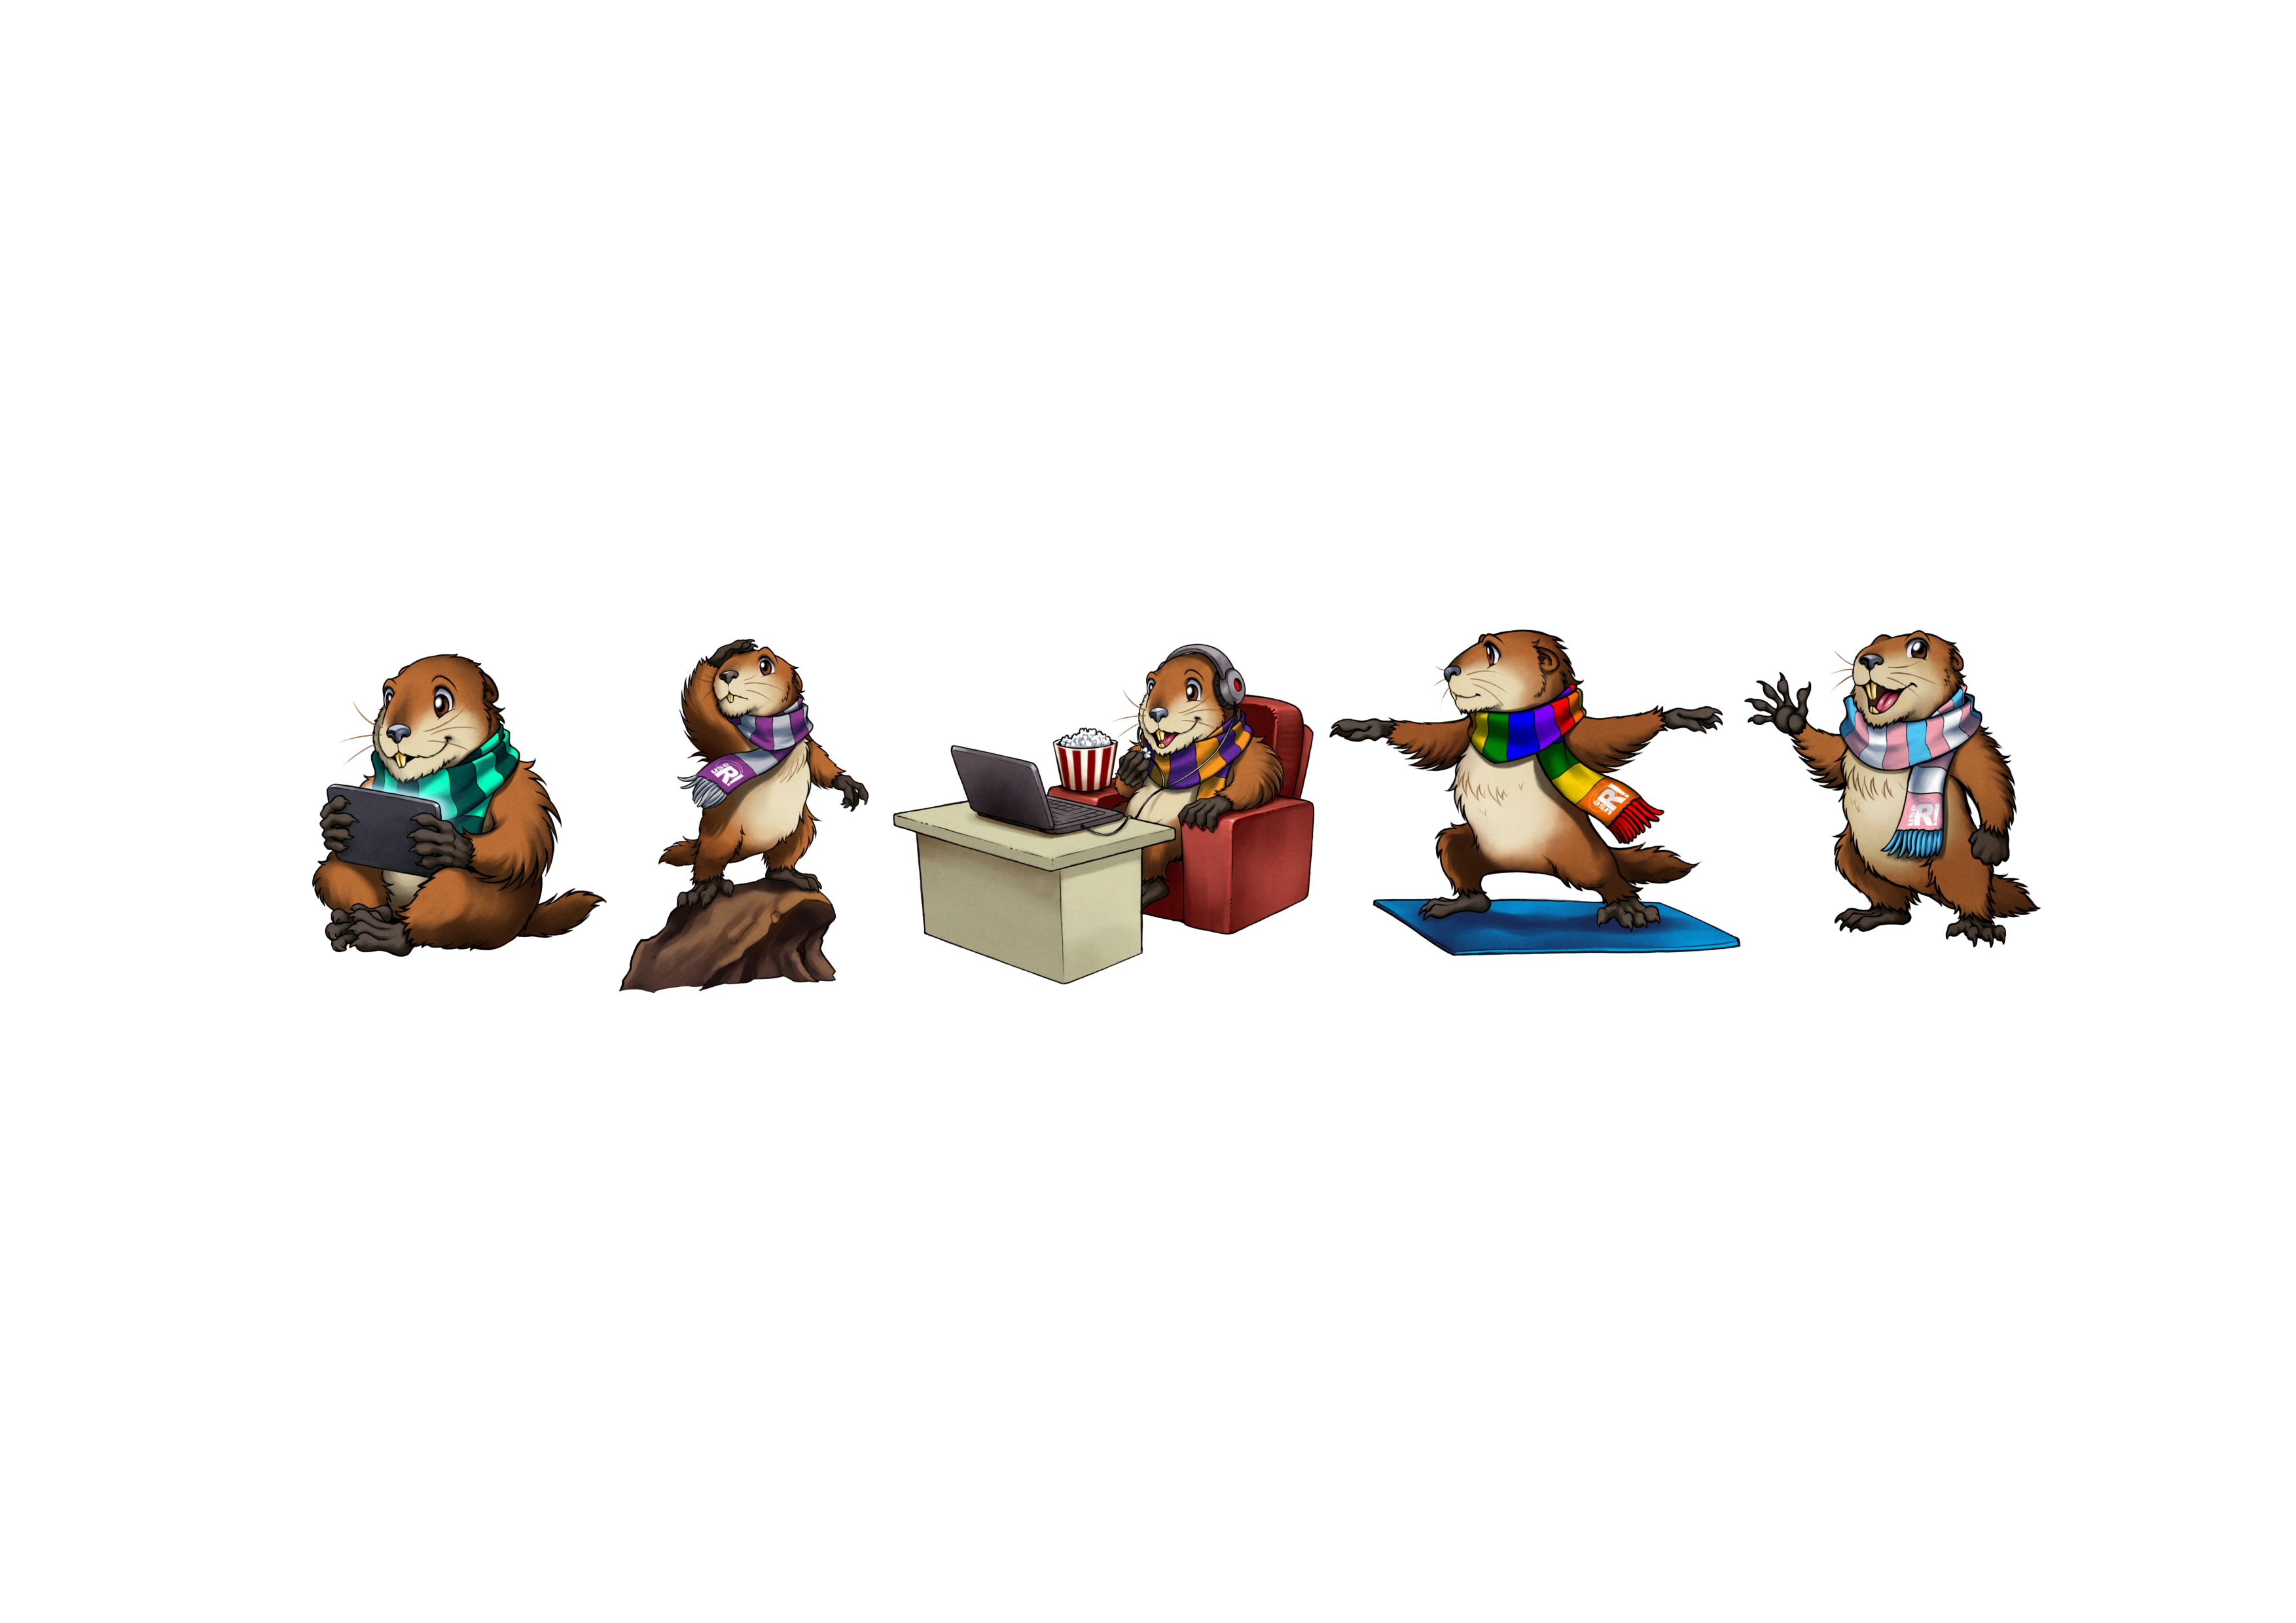
\includegraphics[width=\textwidth]{figs/fig2.pdf}}{
}
\caption{Margot the marmot was the useR! 2021 mascot. To represent the global and inclusive nature of the conference, Margot was drawn using scarves representing the colors of diverse communities of practice that are part of the large R community and specific groups of people we wanted to support explicitly. From left to right: Margot wearing scarves with the colors of MiR (Minorities in R \url{https://mircommunity.com}), R-Ladies \url{https://rladies.org}, AfricaR \url{https://africa-r.org}, and the LGBTQIA+ and transgender communities. Margot was created by Francisco Etchart and is available under a CC-BY-NC-SA license (\url{https://github.com/useRconf/visuals-2021}).}
\label{fig:marmots}
\end{figure}
%alt-text for the figure, to be included in the final PDF: Five marmots with colorful scarves. From left to right: a marmot with a dark and light green scarf from the MiR community is watching her tablet, a marmot with the purple and gray scarf for R-Ladies is stepping on a rock and watches the horizon, a marmot with an orange and purple AfricaR scarf is sitting on a couch watching a film on her laptop with popcorn, a yogi marmot with a rainbow LGBTQIA+ scarf does the warrior pose on her blue mat, and finally, a marmot with a scarf with the pink, light blue and white color of the transgender pride flag waves her hand. 

\section*{Rule 9: Allocate adequate financial resources to support inclusion goals}
\label{rule_financial}

% Rocío: main idea: Need to budget for inclusive practices.
Allocation of resources to support the diversity and inclusion vision and goals has to be intentional and demonstrate true commitment. 
Estimate the costs of these practices and define your priorities in advance (e.g. paying the organizing team, code of conduct training, captioning, accessible software, scholarships).
An online conference might reduce overall costs (e.g. no rental costs for a physical venue), allowing to redirect the money towards inclusive practices. 
When asking for sponsorship, it might be easier to justify supporting concrete actions towards inclusion than making generic requests for funding.

% Rocío: main idea: help take the burden out of participants for more inclusive participation
When determining the registration rates, the socioeconomic context of participants, their career status, and their country of origin—if applicable—should be taken into account  \cite{sarabipourChangingScientificMeetings2021, andalibPostdocQueueLabour2018, kaplanPostdocNot2012}
(see \cite{canelon2021cost} for an example of conversion rates based on country of origin and career status).\linelabel{example-countries}
Resources permitting, enable a `pay what you can' option. You could also aim to have a conference with no registration costs; this could especially apply for online events, but bear in mind that free events have a lower attendance rate than paid events \cite{eventbrite_ultimate_2017}. 
Scholarships to attend the in-person component of the conference are an additional way to boost participation of people from minoritized groups by offering support for travel and lodging expenses.
Design the diversity-related scholarship to be explicit about the groups you want to support and be transparent about the criteria for evaluation to avoid self-selection (refraining from applying). 
To assign these scholarships, conferences usually ask for cover letters or applications, which can be time-consuming and emotionally demanding. 
Simplifying the process of requesting financial support, especially for 
people who lack the time and resources (e.g. because of family responsibilities) could greatly increase their chances of applying for the support. 
Additional aid for attendees could also be offered—e.g. paying for child care or internet connection services for the online component. 
Bear in mind that transferring money internationally could be a cumbersome administrative process and significantly augment the burden of already marginalized groups. Whenever possible, facilitate alternate ways for money transfer (e.g. book flights, hotel reservations, waive conference fees, give gift cards). 

\section*{Rule 10: Make the conference part of a long-term process for inclusion}
\label{rule_process}

% Rocío: main idea: assess how inclusive was the conference
\linelabel{account-3}As conference organizers, one of the key post-conference tasks is to make a final assessment of the achievement of the diversity and inclusion goals. 
You can rely on the diversity goals defined at the beginning of the planning process (\textbf{Rule 1}). 
\linelabel{info}\hl{You will likely be able} to evaluate the outcomes associated with these goals directly from the information collected from the organizing team, speakers, and participants (e.g.\ \hl{city/state/country of origin} or preferred language).
You may have set goals concerning how welcomed and included participants felt during the conference, and need to assess if the implemented practices translated into true inclusion. 
Surveys, focus groups, and informal conversations during and after the conference are good ways to collect this information and great opportunities to receive feedback from the attendees. \linelabel{info2}

% Pass the information
\linelabel{data-share}The feedback received from the participants and the whole assessment of the conference should be documented and shared with \hl{those who helped define the inclusion goals, the attendees, and} future organizers. 
\hl{Ensure that the participants' privacy and anonymity are respected; ask for consent and consider binning/grouping the data into categories when there is a low number of respondents}.\linelabel{data-share2}
Gather and do your best to organize all the documentation produced during the organization process---or even after. Timelines, checklists, budgeting tips, email templates, accessibility checks and guidelines, are a few of many resources that can be shared with your conference successors. 
Create a list with contact information of the members of the organizing team, as well as previous and potential speakers---if they agree to share their contact information---, and pass it along.
For conference series, it could be a good idea to create an official document (e.g. a wiki, knowledge base or similar guide, see for instance \cite{sanchez-tapia_user_2021-2}) that can be used and kept up to date by future organizers.
If you are part of a stable meeting committee (overseeing multiple editions), encourage organizers to follow these Rules and set up new standards for inclusion: be explicit about the inclusive spirit of the conference and the practices that future organizers should commit to when publishing the call for conference organizers and defining the selection criteria. 


\section*{Concluding remarks}

This article recommends changes in conference planning to support greater diversity and inclusion. 
Organizing a conference and implementing inclusive practices are both learning experiences.
As conference organizers ourselves, we started with different levels of clarity about the principles and practices described here, learned many of them together during the organization phase, and learned even more when translating them into ten rules for this paper. 
We hope that they can be useful guidelines to improve diversity and inclusion in your conference, and that you can adapt them, improve them, and share your lessons and experience with as many people as possible. 

Be aware of all the factors that may hinder your efforts for inclusion: systemic discrimination, time or money constraints, geopolitical or public health contexts, or personal issues affecting your organizing team. 
Try to account for these factors as best as you can to set bold yet realistic goals of diversity and inclusion for the conference.
Most importantly, your efforts will enhance the conference experience for all your attendees. 
They will notice the welcoming and inclusive spirit of the conference. 
Remember that inclusive conferences can have lasting impacts in career paths and create a sense of belonging in the community.
That is more than enough motivation to make the effort worth it.


\section*{Authors' contributions}

To list author contributions, we used the high-level contributor roles in the CRediT framework that we considered relevant for this study (project administration, supervision, writing original draft, conceptualization, writing—major reviews and edits, resources, and visualization; \url{http://credit.niso.org}), and additional categories to acknowledge those who shared their own ten simple rules for an inclusive conference without looking at the first draft (i.e. sharing rules), and those who translated the English abstract and the list of rules into different languages.

\begin{itemize}
    \item RJ: Project administration, Supervision, Writing original draft, Conceptualization, Writing---major reviews and edits, Resources, Visualization, Extended abstract translation
    \item AST: Project administration, Supervision, Conceptualization,  Writing---major reviews and edits, Resources, Visualization, Sharing rules, Extended abstract translation
    \item SM: Conceptualization, Writing---major reviews and edits, Resources, Visualization, Sharing rules, Extended abstract translation
    \item YBS: Conceptualization, Writing---major reviews and edits, Resources, Extended abstract translation
    \item HT: Conceptualization, Writing---major reviews and edits, Resources
    \item DHP: Conceptualization, Writing---major reviews and edits, Sharing rules, Extended abstract translation
    \item NSM: Writing---major reviews and edits, Resources, Visualization, Sharing rules, Extended abstract translation
    \item MB: Conceptualization, Extended abstract translation
    \item BA: Writing---major reviews and edits, Resources, Sharing rules, Extended abstract translation
    \item EH: Writing---major reviews and edits, Resources, Sharing rules
    \item LA: Writing---major reviews and edits, Resources
    \item JPN: Writing---major reviews and edits, Visualization
    \item MAC: Writing---major reviews and edits
    \item FM: Writing---major reviews and edits, Extended abstract translation
    \item RG: Writing---major reviews and edits, Resources, Extended abstract translation
    \item SC: Resources, Sharing rules
    \item AE: Sharing rules, Extended abstract translation
    \item AU: Sharing rules
    \item JC: Sharing rules
    \item JR: Conceptualization, Writing---major reviews and edits, Visualization, Extended abstract translation
\end{itemize}


\section*{Acknowledgments}
The authors of this piece would like to thank every single member of the organizing team of useR! 2021 (\url{https://user2021.r-project.org/about/global-team}) for their valuable contribution to an inclusive conference experience and the R Foundation for trusting us with the organization of useR! 2021 and supporting us through the process. Special thanks to Saranjeet Kaur and gwynn sturdevant for suggestions to previous versions of the manuscript, and Francisco Etchart for his help with the Marmot figures. We would also like to thank Arjun Krishnan, Julia Ganz, Ingo Braasch, Susan Ewart, and Hilda Mejia-Abreu for their feedback on the manuscript. In addition to some of the authors (listed in the Translated Abstracts section of Supporting Information), we would like to acknowledge the following contributors for translating our extended abstract: Koki Tsuyuzaki and Kozo Nishida [Japanese], KwangChun Lee [Korean], Arjun Krishnan [Tamil], Kewalin Samart, Natnaree Yolnava, and Wanprakai Kaewphrae [Thai].
The comments of the anonymous reviewers contributed to the improvement of the manuscript and we thank them for that.

\section*{Funding}

JR is funded by start-up award from Michigan State University (MSU); publication costs were waived because of MSU’s institutional partnership with PLoS. HT was supported by the Engineering and Physical Sciences Research Council [EPSRC EP/V052128/1] during the preparation of this article.

The organization of useR! 2021---which inspired this work---was largely a volunteer effort (from many people including all the authors), but stipends were given from the conference funds for some specific roles.
AE, AU, AST, BA, JC, JPNG, MAC, NM, RG, RJ, SM, and YBS received stipends for roles that include code of conduct team, zoom host, and diversity and social program leads.

The funders had no role in study design, decision to publish, or preparation of the manuscript.


\section*{Data availability}
For the purpose of open access, the authors have applied a Creative Commons Attribution (CC BY) license to any author accepted manuscript version arising from this submission. The manuscript, figures, supplementary material, and supporting docs are available at: https://github.com/rociojoo/Ten-simple-rules-inclusive-conference.

% \nolinenumbers

% % Either type in your references using
% % \begin{thebibliography}{}
% % \bibitem{}
% % Text
% % \end{thebibliography}
% %
% % or
% %
% % Compile your BiBTeX database using our plos2015.bst
%\bibliography{community-science}
% % style file and paste the contents of your .bbl file
% % here. See http://journals.plos.org/plosone/s/latex for 
% % step-by-step instructions.
% % % 
\begin{thebibliography}{10}

\bibitem{arendDisparityConferenceRegistration2019}
Arend ME, Bruijns SR.
\newblock Disparity in Conference Registration Cost for Delegates from Low- and
  Middle-Income Backgrounds.
\newblock African Journal of Emergency Medicine. 2019;9(3):156--161.
\newblock doi:{10.1016/j.afjem.2019.01.016}.

\bibitem{biggsAcademicConferenceChilly2018}
Biggs J, Hawley PH, Biernat M.
\newblock The {{Academic Conference}} as a {{Chilly Climate}} for {{Women}}:
  Effects of {{Gender Representation}} on {{Experiences}} of {{Sexism}},
  {{Coping Responses}}, and {{Career Intentions}}.
\newblock Sex Roles. 2018;78(5):394--408.
\newblock doi:{10.1007/s11199-017-0800-9}.

\bibitem{depickerRethinkingInclusionDisability2020a}
De~Picker M.
\newblock Rethinking Inclusion and Disability Activism at Academic Conferences:
  Strategies Proposed by a {{PhD}} Student with a Physical Disability.
\newblock Disability \& Society. 2020;35(1):163--167.
\newblock doi:{10.1080/09687599.2019.1619234}.

\bibitem{irishIncreasingParticipationUsing2020}
Irish JEN.
\newblock Increasing Participation: Using the Principles of Universal Design to
  Create Accessible Conferences.
\newblock Journal of Convention \& Event Tourism. 2020;21(4):308--330.
\newblock doi:{10.1080/15470148.2020.1814469}.

\bibitem{sanchez-tapia_user_2021-2}
{S{\'a}nchez-Tapia} A, Tamir N, Moy~Das S, Bellini~Saibene Y, Joo R, Morandeira
  N, et~al.. {{useR}}! {{Knowledgebase}}; 2021.
\newblock https://rconf.gitlab.io/userknowledgebase/.

\bibitem{r_core_team_2021}
{R Core Team}. R: A Language and Environment for Statistical Computing; 2021.
\newblock Available from: \url{https://www.R-project.org/}.

\bibitem{crenshawDemarginalizingIntersectionRace1989}
Crenshaw K.
\newblock Demarginalizing the {{Intersection}} of {{Race}} and {{Sex}}: A
  {{Black Feminist Critique}} of {{Antidiscrimination Doctrine}}, {{Feminist
  Theory}} and {{Antiracist Politics}}.
\newblock University of Chicago Legal Forum. 1989;1989:139.

\bibitem{numfocus_discover_2021}
{NumFOCUS Diversity \& Inclusion in Scientific Computing (DISC) Program}.
  {{DISCOVER Cookbook}} {$\cdot$} {{Diverse}} \& {{Inclusive Spaces}} and
  {{Conferences}}; 2021.
\newblock https://discover-cookbook.numfocus.org/.

\bibitem{favaroYourScienceConference2016}
Favaro B, Oester S, Cigliano JA, Cornick LA, Hind EJ, Parsons ECM, et~al.
\newblock Your {{Science Conference Should Have}} a {{Code}} of {{Conduct}}.
\newblock Frontiers in Marine Science. 2016;0.
\newblock doi:{10.3389/fmars.2016.00103}.

\bibitem{auroraHowRespondCode2019}
Aurora V, Gardiner M.
\newblock How to {{Respond}} to {{Code}} of {{Conduct Reports}}. {{A}}
  Practical Step-by-Step Guide to Handling Code of Conduct Issues.
\newblock {Frame Shift Consulting LLC}; 2019.
\newblock Available from:
  \url{https://frameshiftconsulting.com/resources/code-of-conduct-book/}.

\bibitem{charlton_nothing_1998}
Charlton JI.
\newblock Nothing about us without us.
\newblock University of California Press; 1998.

\bibitem{werner_nothing_1998}
Werner D, Thuman C, Maxwell J.
\newblock Nothing about us without us.
\newblock Developing innovative technologies for, by and with disabled persons
  Palo Alto: Healthwrights. 1998;.

\bibitem{hongGroupsDiverseProblem2004}
Hong L, Page SE.
\newblock Groups of Diverse Problem Solvers Can Outperform Groups of
  High-Ability Problem Solvers.
\newblock Proceedings of the National Academy of Sciences.
  2004;101(46):16385--16389.
\newblock doi:{10.1073/pnas.0403723101}.

\bibitem{costanzachockDesign2020}
{Costanza-Chock} S.
\newblock Design Justice: Community-Led Practices to Build the Worlds We Need.
\newblock Braman S, editor. Information {{Policy}}. {Cambridge, MA, USA}: {MIT
  Press}; 2020.

\bibitem{dwyerNoticeWhoScience2021}
Dwyer JR.
\newblock Notice Who the Science System Honours, and How.
\newblock Nature. 2021;595(7865):30--30.
\newblock doi:{10.1038/d41586-021-01785-3}.

\bibitem{swartzScienceValueDiversity2019}
Swartz TH, Palermo AGS, Masur SK, Aberg JA.
\newblock The {{Science}} and {{Value}} of {{Diversity}}: Closing the {{Gaps}}
  in {{Our Understanding}} of {{Inclusion}} and {{Diversity}}.
\newblock The Journal of Infectious Diseases. 2019;220(Supplement\_2):S33--S41.
\newblock doi:{10.1093/infdis/jiz174}.

\bibitem{wongBuildDiversityScience2020}
Wong VNL, Shaw JD.
\newblock Build Diversity among Science Prize Winners.
\newblock Nature. 2020;580(7802):185--185.
\newblock doi:{10.1038/d41586-020-01033-0}.

\bibitem{dignazioUnicornsJanitorsNinjas2020}
D'Ignazio C, Klein L.
\newblock 5. {{Unicorns}}, {{Janitors}}, {{Ninjas}}, {{Wizards}}, and {{Rock
  Stars}}.
\newblock In: Data {{Feminism}}. {PubPub}; 2020.Available from:
  \url{https://data-feminism.mitpress.mit.edu/pub/2wu7aft8/release/2}.

\bibitem{spitschanVideoGrantProposals2021}
Spitschan M, Yehudi Y, Acion L.
\newblock Video Grant Proposals Could Be Exclusionary.
\newblock Nature. 2021;592(7852):26--26.
\newblock doi:{10.1038/d41586-021-00862-x}.

\bibitem{ross_everyday_2020}
Ross HJ.
\newblock Everyday {{Bias}}: {{Identifying}} and {{Navigating Unconscious
  Judgments}} in {{Our Daily Lives}}.
\newblock {Rowman \& Littlefield}; 2020.

\bibitem{andersson_implicit_2019}
Andersson ER, Hagberg C, H{\"a}gg S. Implicit Bias Is Strongest When Assessing
  Top Candidates; 2019.

\bibitem{cheng2020x+}
Cheng E.
\newblock X+ Y: A Mathematician's Manifesto for Rethinking Gender.
\newblock Basic Books; 2020.

\bibitem{burfordHomelinessMeantHaving2020}
Burford J, Bosanquet A, Smith J.
\newblock `{{Homeliness}} Meant Having the Fucking Vacuum Cleaner out': The
  Gendered Labour of Maintaining Conference Communities.
\newblock Gender and Education. 2020;32(1):86--100.
\newblock doi:{10.1080/09540253.2019.1680809}.

\bibitem{light_gender_2022}
Light AE, {Benson-Greenwald} TM, Diekman AB.
\newblock Gender Representation Cues Labels of Hard and Soft Sciences.
\newblock Journal of Experimental Social Psychology. 2022;98:104234.

\bibitem{jooKeepOnlineOption2021}
Joo R.
\newblock Keep Online Option at Conferences \textemdash{} It Makes Them More
  Inclusive.
\newblock Nature. 2021;598(7880):257--257.
\newblock doi:{10.1038/d41586-021-02752-8}.

\bibitem{woolstonLearningLoveVirtual2020}
Woolston C.
\newblock Learning to Love Virtual Conferences in the Coronavirus Era.
\newblock Nature. 2020;582(7810):135--136.
\newblock doi:{10.1038/d41586-020-01489-0}.

\bibitem{ninerBetterWhomLeveling2021}
Niner HJ, Wassermann SN.
\newblock Better for {{Whom}}? Leveling the {{Injustices}} of {{International
  Conferences}} by {{Moving Online}}.
\newblock Frontiers in Marine Science. 2021;0.
\newblock doi:{10.3389/fmars.2021.638025}.

\bibitem{roosOnlineConferencesNew2020}
Roos G, Ol{\'a}h J, Ingle R, Kobayashi R, Feldt M.
\newblock Online Conferences \textendash{} {{Towards}} a New (Virtual) Reality.
\newblock Computational and Theoretical Chemistry. 2020;1189:112975.
\newblock doi:{10.1016/j.comptc.2020.112975}.

\bibitem{levitisCenteringInclusivityDesign2021}
Levitis E, {van Praag} CDG, Gau R, Heunis S, DuPre E, Kiar G, et~al.
\newblock Centering Inclusivity in the Design of Online
  Conferences\textemdash{{An OHBM}}\textendash{{Open Science}} Perspective.
\newblock GigaScience. 2021;10(8).
\newblock doi:{10.1093/gigascience/giab051}.

\bibitem{sarabipourChangingScientificMeetings2021}
Sarabipour S, Khan A, Seah YFS, Mwakilili AD, Mumoki FN, S{\'a}ez PJ, et~al.
\newblock Changing Scientific Meetings for the Better.
\newblock Nature Human Behaviour. 2021;5(3):296--300.
\newblock doi:{10.1038/s41562-021-01067-y}.

\bibitem{salibaGettingGripsOnline2020}
Saliba M.
\newblock Getting to Grips with Online Conferences.
\newblock Nature Energy. 2020;5(7):488--490.
\newblock doi:{10.1038/s41560-020-0656-z}.

\bibitem{gichoraTenSimpleRules2010a}
Gichora NN, Fatumo SA, Ngara MV, Chelbat N, Ramdayal K, Opap KB, et~al.
\newblock Ten {{Simple Rules}} for {{Organizing}} a {{Virtual
  Conference}}\textemdash{{Anywhere}}.
\newblock PLOS Computational Biology. 2010;6(2):e1000650.
\newblock doi:{10.1371/journal.pcbi.1000650}.

\bibitem{bajpai_towards_2021}
Bajpai V, Hohlfeld O, Crowcroft J, Keshav S.
\newblock Towards Climate-Friendly Internet Research (Dagstuhl Seminar 21272).
\newblock In: Dagstuhl Reports. vol.~11. Schloss Dagstuhl-Leibniz-Zentrum
  f{\"u}r Informatik; 2021.

\bibitem{trianaDoesOrderFacetoFace2012}
Triana MdC, Kirkman BL, Wagstaff MF.
\newblock Does the {{Order}} of {{Face}}-to-{{Face}} and
  {{Computer}}-{{Mediated Communication Matter}} in {{Diverse Project Teams}}?
  An {{Investigation}} of {{Communication Order Effects}} on {{Minority
  Inclusion}} and {{Participation}}.
\newblock Journal of Business and Psychology. 2012;27(1):57--70.

\bibitem{blackEngenderingBelongingThoughtful2020}
Black AL, Crimmins G, Dwyer R, Lister V.
\newblock Engendering Belonging: Thoughtful Gatherings with/in Online and
  Virtual Spaces.
\newblock Gender and Education. 2020;32(1):115--129.
\newblock doi:{10.1080/09540253.2019.1680808}.

\bibitem{priceAccessImaginedConstruction2009}
Price M.
\newblock Access {{Imagined}}: The {{Construction}} of {{Disability}} in
  {{Conference Policy Documents}}.
\newblock Disability Studies Quarterly. 2009;29(1).
\newblock doi:{10.18061/dsq.v29i1.174}.

\bibitem{marks2021meeting}
Marks GS, Solomon C, Whitney KS.
\newblock Meeting frameworks must be even more inclusive.
\newblock Nature Ecology \& Evolution. 2021;5(5):552--552.

\bibitem{pun_dos_2016}
Pun K. Dos and Don'ts on Designing for Accessibility - {{Accessibility}} in
  Government; 2016.
\newblock
  https://accessibility.blog.gov.uk/2016/09/02/dos-and-donts-on-designing-for-accessibility/.

\bibitem{sanchez-tapia_user_2021}
{S{\'a}nchez-Tapia} A, Hare L, Ch{\'a}vez J, Canel{\'o}n S, Hug~Peter D.
  {{useR}}! 2021 {{Accessibility}} Guidelines; 2021.

\bibitem{chavez_preparing_2021}
Ch{\'a}vez J. Preparing for an {{Accessible Online Conference}}; 2021.
\newblock
  https://user2021.r-project.org/blog/2021/02/17/preparing-for-an-accessible-conference//.

\bibitem{sanchez-tapia_making_2021}
{S{\'a}nchez-Tapia} A, Hare L, Ch{\'a}vez J, Mortara S, Joo R. Making
  Accessible Presentations at {{useR}}! 2021: The Story behind the Scenes;
  2021.
\newblock
  https://user2021.r-project.org/blog/2021/12/07/accessibility\_awards\_interview//.

\bibitem{joo_how_2021}
Joo R, Canel{\'o}n S, Ch{\'a}vez J, {S{\'a}nchez-Tapia} A. How to Improve
  Conference Accessibility for Screen-Reader Users\textemdash an Interview with
  {{Liz Hare}}; 2021.
\newblock
  https://user2021.r-project.org/blog/2021/11/04/accessibility\_interview\_liz\_hare//.

\bibitem{amanoTenTipsOvercoming2021}
Amano T, Rios~Rojas C, Boum~II Y, Calvo M, Misra BB.
\newblock Ten tips for overcoming language barriers in science.
\newblock Nature Human Behaviour. 2021;5(9):1119--1122.
\newblock doi:{10.1038/s41562-021-01137-1}.

\bibitem{hallDesigningDiversityInclusion2019}
Hall B. Designing a Diversity and Inclusion ({{D}}\&{{I}}) Communications
  Strategy; 2019.
\newblock Available from:
  \url{https://www.interactsoftware.com/blog/diversity-inclusion-communications-strategy/}.

\bibitem{andalibPostdocQueueLabour2018}
Andalib MA, Ghaffarzadegan N, Larson RC.
\newblock The {{Postdoc Queue}}: A {{Labour Force}} in {{Waiting}}.
\newblock Systems Research and Behavioral Science. 2018;35(6):675--686.
\newblock doi:{10.1002/sres.2510}.

\bibitem{kaplanPostdocNot2012}
Kaplan K.
\newblock Postdoc or Not?
\newblock Nature. 2012;483(7390):499--500.
\newblock doi:{10.1038/nj7390-499a}.

\bibitem{canelon2021cost}
Canelón S. useR!2021 Cost Conversion Tool: Cost Conversion Tool; 2021.
\newblock Available from:
  \url{https://spcanelon.github.io/useR2021-cost-conversion-tool}.

\bibitem{eventbrite_ultimate_2017}
{Eventbrite}. The Ultimate Way to Reduce No-Shows at Free Events;.
\newblock Available from:
  \url{https://www.eventbrite.com/blog/asset/ultimate-way-reduce-no-shows-free-events/}.

\end{thebibliography}

\section*{Supporting Information}

Supporting Information 1. Abstract and list of rules in multiple languages: Arabic, French, German, Italian, Japanese, Korean, Portuguese, Spanish, Tamil, and Thai.

Supporting Information 2. Rules proposed in the process of shaping these ten simple rules. 




\end{document}

